\section{Livello rete}
Mette in comunicazione gli \textbf{host}. È implementato in ogni livello. È colui che trasporta i vari \textit{segmenti} (mandati dal livello di trasporto) e li trasforma in \textbf{datagrammi} lato mittente, mentre il destinatario consegna i \textbf{datagrammi} al livello trasporto, quindi \textit{segmenti}.
Ci sono due funzioni principali a livello di rete 
\begin{itemize}
  \item \textbf{Inolto o forwarding}: è un'azione locale, definisce qual è il percorso per il destinatario desegnato, dipende dall'\textbf{instradamento}, l'\textit{instradamento} aggiorna i percorsi e li comunica all'\textit{inoltro}.
  \item \textbf{Instradamento o routing}: Consiste nel trovare (non come) la strada migliore per andare da una sorgente a una destinazione.
\end{itemize}

\subsection{Architettura del router}
Nel router abbiamo due compontenti, una si occupa dell'instradamneto e una si occupa dell'inoltro. 
In alto abbiamo la componente che gestisce l'instradamento con un \textbf{algoritmo di instradamento}, sotto abbiamo la componente che gestisce l'inoltro, che avrà una tabella con tutte le informazioni mandate dalla componente di instradamento. 

Il primo piano si chiamata \textbf{piano di controllo}. 
Il secondo piano si chiamata \textbf{piano dei dati} diviso in:
\begin{itemize}
  \item \textbf{Porte di ingresso}: porte logiche, non sono le porte fisiche, è uno stream di dati \textit{socket}. 
    Ha il livello fisico (ricezione di dati), livello di collegamento (ethernet) e livello di rete col commutazione decentralizzata: determina la porta d'uscita dei pacchetti tramite la tabella d'inoltro, nel caso in cui arrivano tanti datagrammi che il router non riesce a manipolare man mano crea un \textit{buffer di accodamento} dove memorizza i pacchetti. 
  \item \textbf{Struttura di commutazione}: inizialmente era un computer che manipolava i dati e aveva le porte come periferiche (\textit{Commutazione in memoria}), ora usiamo la \textbf{commutazione tramite bus}:
    le porte d'ingresso gestiscono l'indirizzamento del pacchetto, manipolano loro la circuteria per l'instradamento. 
    La soluzione ideale è \textbf{crossbar switch}, sono percorsi in parallelo con $2n$ bus che collegano $n$ porte d'ingresso a $n$ porte d'uscita. 
  \item \textbf{Porte di uscita}: porte logiche, non sono le porte fisiche, è uno stream di dati \textit{socket}. Hanno gli stessi livelli della \textit{porta d'ingresso} ma in modo speculare. 
    Le funzionalità di \textit{livello rete} sono: \textbf{funzionalità di accodamento} che riframmenta i pacchetti nel caso in cui il \textit{livello di collegamento} ha un \textit{MTU} inferiore al precedente. 
\end{itemize}

\subsubsection{Tabelle di inoltro}


\subsection{Protocollo internet: IP}
Il protocollo \textbf{IP} (sia in versione 4 che in versione 6) stabilisce:
\begin{itemize}
  \item Convenizioni di indirizzamento
  \item Formato dei datagrammi 
  \item La manipolazione dei pacchetti
\end{itemize}
Il protocollo \textbf{ICMP}, dipendente dal protocollo \textit{IP}:
\begin{itemize}
  \item Notifica gli errori
  \item Segnalazione del router
\end{itemize}

\subsubsection{Formato dei datagrammi}
Lungo 32 bit. Abbiamo i seguenti campi:
\begin{enumerate}
  \item \begin{enumerate}
      \item \textbf{Versione} del protocollo (4 o 6)
      \item \textbf{Lunghezza intestazione}, variabile 
      \item \textbf{Tipo di servizio} quanto è importante il datagramma (non molto utilizzato)
      \item \textbf{Lunghezza del datagramma}
  \end{enumerate}
  \item \begin{enumerate}
      \item \textbf{Identificatore a 16 bit}: 
      \item \textbf{flag}:
      \item \textbf{Spiazzamento di frammentazione a 13bit}:
  \end{enumerate}
  \item \begin{enumerate}
      \item \textbf{Tempo di vita residuo}: \textit{TTL - Time to live}, quanti router può attraversa il datagramma, il datagramma nasce con un tempo di vita previsto, a ogni passaggio viene decrementato di 1, quando il \textit{TTL} arriva a 0 il router elimina il pacchetto.  
      \item \textbf{Protocollo di livello superiore}: specifica quale \textit{protocollo} stiamo utilizzando a livello di \textit{trasporto}, per sapere a quale servizio del \textit{sistema operativo} mandare i pacchetti.
      \item \textbf{Checksum} della sola intestazione, stesso algoritmo del protocollo \textit{UDP}, chiamato \textbf{checksum internet}, non comprendere il campo \textit{Dati}. Viene calcolata da ogni \textit{router} in cui passa. 
  \end{enumerate}
  \item \textbf{Indirizzo IP origine}
  \item \textbf{Indirzzo IP destinazione}
  \item \textbf{Campi opzionali}
  \item \textbf{Dati}
\end{enumerate}

\subsubsection{frammentazione dei datagrammi IP}
L'unità massima di trasmissione (\textbf{MTU}) è la quantità massima di dati che possono passare in quel determinato \textit{livello di collegamento}. 
I \textbf{datagrammi IP} vengono frammentati in \textit{datagrammi} più piccoli. 

\subsection{IPv4, Protocollo IP versione 4}
Ogni \textit{interfaccia di host} e \textit{router} hanno un \textbf{indirizzo IP univoco da 32 bit}. 
L'\textbf{interfaccia} è il confine tra host e collegamento fisico, i \textit{router} devono avere almeno due collegamenti fisici  e per ogni \textit{interfaccia} è associato un \textbf{indirizzo IP}. 

\subsubsection{Sottorete}
L'\textit{indirizzo IP} è diviso in due parti:
\begin{itemize}
  \item \textbf{Parte di sottorete}: bit di alto ordine. 
  \item \textbf{Parte dell'host}: bit di basso ordine. 
\end{itemize}
Una sottorete è definita anche come \textit{reti IP}. 

\subsubsection{Assegnazione indirizzi internet CIDR}
\textbf{CIDR}: Classes InterDomain Routing \\ 
L'\textit{indirizzo IP} viene diviso in $a.b.c.d/x$ dove $x$ è un numero in bit che definisce la \textbf{maschera di rete}. 
Facendo $32 - x$ avremo il numero di bit \textit{"liberi"} per la \textit{sottorete}. 
\subsubsection*{Esempio}
$200.23.16.0/23$ diventa $11001000.000101111.0001000\textbf{0}.\textbf{00000000}$ dove la parte in grassetto è \textbf{parte di host}, mentre il resto è \textbf{parte di sottorete}. Avendo $x=23$ faremo $32-23 = 9$, quindi avremo correttamente $9$ bit di \textbf{parte di host}. 

\subsubsection{Indirizzamento}
Convenizioni:
\begin{itemize}
  \item \textbf{Broadcast}: tutti i bit della \textbf{parte di host} posti a $1$. Il datagrammo viene consegnato a tutti gli host della sottorete. 
  \item \textbf{Identificativo della rete}: Tutti i bit della \textbf{parte di host} è posta a $0$. Indirizzo della rete.
  \item \textbf{Identificatore del router}: solitamente il primo indirizzo disponibile (dopo quelli \textbf{riservati}) è del \textit{router}.
\end{itemize}

\subsubsection{Netmask}
Sequenza di 32 bit associato ad un indirizzo per l'individuazione del prefisso di rete e parte di host.  \\ 
I bit che valgono $1$ indentificano la \textit{parte di rete} e quelli che valgono $0$ indentificano la \textit{parte di host}. \\  
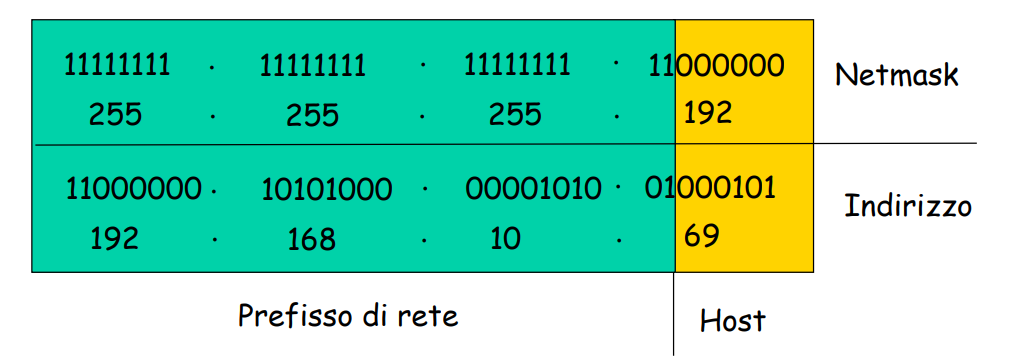
\includegraphics[width=\textwidth]{./img/netmask.png} 

\subsubsection{Inoltro dei pacchetti: Host}
Operazioni che fa:
\begin{enumerate}
  \item Verifica se il destinatario è nella stessa sottorete: \textit{AND} tra il proprio indirizzo e la propria \textit{netmask}, \textit{AND} tra l'indirizzo di destinazione e la propria \textit{netmask}, verifica se sono uguali.
  \item Se è sulla stessa \textit{sottorete} invia direttamente all'host. Se non è nella stessa \textit{sottorete} invia al router.  
\end{enumerate}

\subsubsection{Inoltro dei pacchetti: router}

\subsubsection{Come ottenere un blocco di indirizzi IP}
Bisogna contattare il proprio \textbf{ISP} e ottenere la divisione in otto blocchi uguali di inidirizzi contigui. 

\subsubsection{Come ottenere un singolo indirizzo}
Due approcci:
\begin{itemize}
  \item \textbf{configurazione manuale}: si imposta manualmente l'indirizzo IP alla macchina. 
  \item \textbf{DHCP}: Dynamic Host Configuration Protocol, assegna automaticamente un indirizzo IP una volta connesso in rete.  
\end{itemize}

\subsubsection*{DHCP}
È una funzionalità di livello rete ma gestita da un processo a livello applicativo che utilizza delle socket UDP, porta con numero 67, mentre i client aprono la porta 68 con indirizzo IP $0.0.0.0$. \\ 
Il client appena inserito sulla rete non ha, giustamente, indirizzo IP e non conosce l'indirizzzo IP del server DHCP, quindi il client invia un messaggio \textit{broadcast} sulla porta 67, cercando un server DHCP. \\ 
Consente di ottenere \textbf{dinamicamente} gli indirizzi IP degli \textit{host}. Non assegna obbligatoriamente lo stesso IP all'host, varia in base a quelli che ha disponibile. \\ 
\begin{enumerate}
  \item \textbf{DHCP discover} da parte degli host, un messaggio broadcast a tutta la rete alla ricerca di un \textbf{server DHCP} 
  \item \textbf{DHCP offer}: il \textit{server DHCP} offre un indirizzo IP all'host. 
  \item \textbf{DHCP request}: l'host accetta l'indirizzo ip proposto dal \textit{server DHCP}. 
  \item \textbf{DHCP ack}: il \textit{server DHCP} invia l'ack di conferma. 
\end{enumerate}
